\documentclass[10pt]{article}
\usepackage[margin=1.5cm]{geometry}
\usepackage{graphicx,hyperref,booktabs,amsmath,amssymb}
\hypersetup{colorlinks=true,urlcolor=blue}
\setlength{\parindent}{0pt}
\setlength{\parskip}{6pt}
\begin{document}
\begin{center}
{\Large Exact retained-point membership: $8\to4$ and $16\to5$}\\[4pt]
17 November 2026 \quad Research PR4567 \quad Unsigned producer certificates
\end{center}

The actual P-256 retained signed-point membership ideal has regularity8
versus4 on18points, and16 versus5 on42points, under the same degree-compatible
Buchberger--M\"oller preprocessing. The full relation-system goal remains
unmet: these are membership ideals, not complete group-law systems.

Target: \texttt{icv1-fp256-t89188191154553853111372247798585809583-f188c491}.
The factor base, both target signs, original FB1 encoding and fixed seed are
unchanged. Extra coordinates are unique auxiliary-chain abscissae; there is
no auxiliary sign cover or target-log transport.

\begin{center}
\begin{tabular}{llrrr}
\toprule
Depth & Factor base & Signed points & Variables dense/chain & $D$ dense/chain\\
\midrule
2 & FB1hb6856918fe35 & 4 & 2/3 & 3/3\\
4 & FB1h2704fe49495e & 18 & 2/5 & 8/4\\
5 & FB1h8bc0ab2ed2af & 42 & 2/6 & 16/5\\
\bottomrule
\end{tabular}
\end{center}
One fixed base per depth. Exact native component checks, no statistical or
timing data. Neutral depth2 control retained. Claim
\texttt{PCC-20261117-ed749f}; no independent signed/Lean standing.

\begin{center}
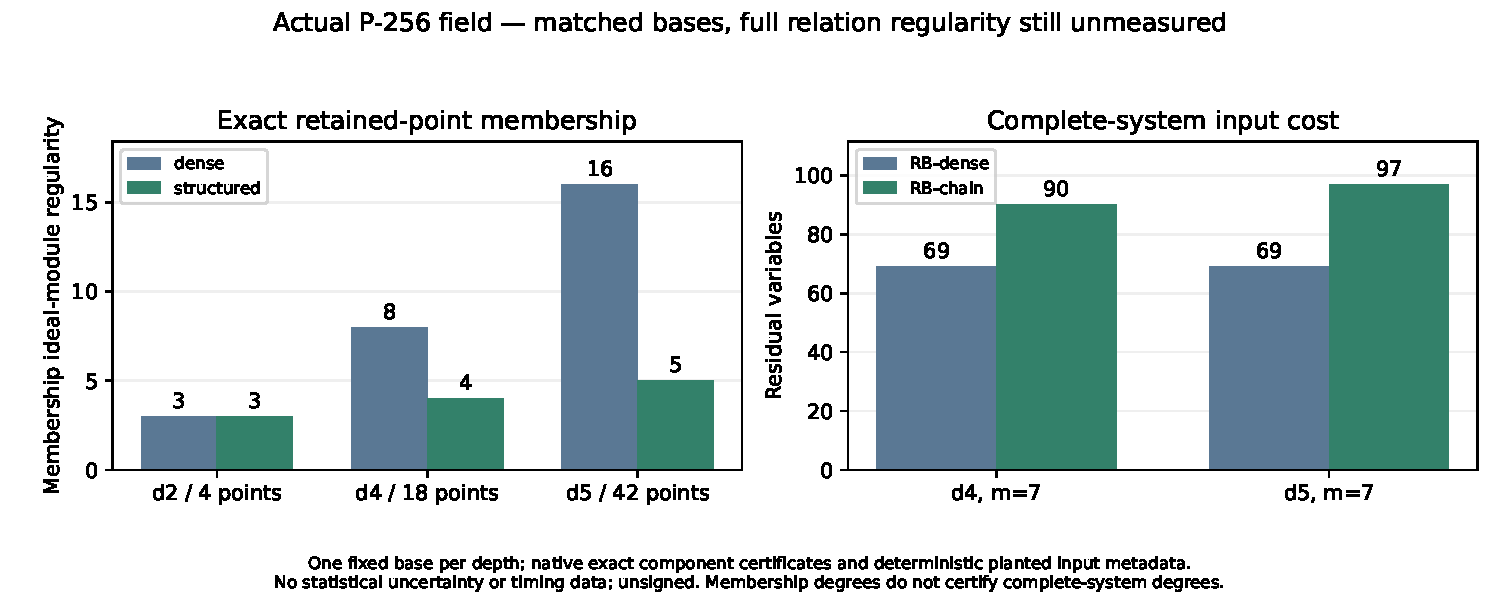
\includegraphics[width=\linewidth]{retained-comparison.pdf}
\end{center}

\textbf{What the certificate checks.}
Every point is retained and rational. The payload supplies generators,
their homogenization, standard monomials and Hilbert numerator. Checks:
point vanishing, all nontrivial S-pairs, product criterion, independent
evaluation rank, divisor-closed footprint and complete border. Direct
homogeneous S-pairs have H-free leading terms. Thus the quotient is graded
free over $\mathbb F_p[H]$, CM of dimension1. The highest standard-monomial
degree$r$ gives quotient regularity$r$ and ideal regularity$D=r+1$.

For depth4 the Hilbert numerators are
$[1,2,3,3,3,3,2,1]$ and $[1,5,8,4]$, giving $D=8$ and4.
This is not a final-basis-degree proxy. Twelve signed/abscissa cells and
36corrupt-certificate controls pass; fresh replay is byte-identical.

The N-dimensional quotient evaluates isomorphically onto N distinct points,
so it is their radical vanishing ideal over the algebraic closure too.
Projection and unique chain lift give the same affine point algebra. The
old unpruned fibre's extra extension points are absent.

\newpage
\textbf{Same point algebra, complete relation degree still open}
\begin{center}
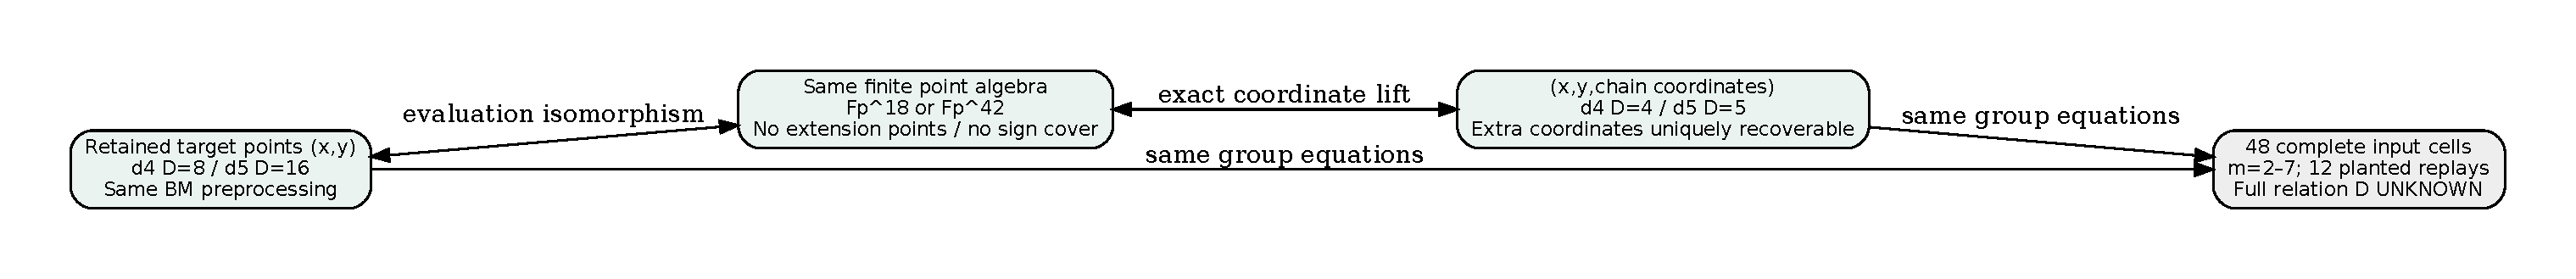
\includegraphics[width=\linewidth]{retained-flow.pdf}
\end{center}

The bridge exports48paired complete inputs: depths4/5, $m=2$--7,
planted/unplanted, RB-dense/RB-chain. All group-law equations are retained;
only point membership is replaced. Both arms use the same frozen linear
preprocessor. Twelve planted target identities are replayed with GMP/OpenSSL;
24original/reconstructed systems satisfy all equations. Unplanted targets
were exported, not solved. Claim \texttt{PCC-20261117-dc7483}, unsigned.

\begin{center}
\begin{tabular}{lrrrr}
\toprule
Planted m7 input & Residual variables & Equations & Terms & Input degree\\
\midrule
d4 RB-dense & 69 & 212 & 1048 & 8\\
d4 RB-chain & 90 & 240 & 1230 & 3\\
d5 RB-dense & 69 & 212 & 1300 & 16\\
d5 RB-chain & 97 & 303 & 2532 & 4\\
\bottomrule
\end{tabular}
\end{center}
These are input counts, not full regularities or solve costs. Setup/verification
GMP API counters and base-construction certificates are recorded separately;
they are not field-equivalent solve counts. Extra variables and terms are
charged explicitly. RAM, disk traffic, complete solve cost and original
depth8 validation remain open. m2 equations are materialized; higher-m
payloads are reproducible from source/cache and manifest hashes.

\textbf{Complete-system qualification failures.}
The official CoCoA5.4.0 archive matches vendor SHA256. A known-answer unit
passes at the exact256-bit modulus: CI ideal4/quotient3 and linear ideal1/
quotient0. All four old frozen complete-system cells time out at45seconds,
exit124, with no admitted certificate. Three print partial ideal assertions
6,8,13 before the Betti stage fails to finish; the fourth prints only start.
Those lines are unadmitted, not accepted values. Claim
\texttt{PCC-20261117-0033dc}; all failures retained, no retry.

The strict native-algebra bound is240seconds: known-answer probe, four
45-second cells, and two25-second membership invocations. Serialization/
build checks are development setup. No new public-service request or timing
experiment. Initial partial software download and compiler error retained.

\textbf{Reproduce and continue.}
\texttt{run\_retained\_checks.sh FRESH\_DIR} reproduces exact component checks.

\texttt{build\_retained\_bridge.sh FRESH\_DIR} reconstructs paired inputs.
C++20/O2/Wall/Wextra/Werror, GMP/OpenSSL, offline. Wrapper constituent
commands ran; shell syntax checked without another qualification run.

Full completion still requires a complete-ideal certificate and original
$m=2$--7/depth8 validation. The unexecuted successor in
\texttt{FINITE\_POINT\_ROUTE.md} examines complete projective addition and
H-torsion bounds. Comparing membership degrees or two upper bounds cannot
establish a full2x reduction. No end-to-end speedup or novelty is asserted.

Sources: Abbott--Kreuzer--Robbiano, \emph{Computing Zero-Dimensional Schemes},
Theorem3.1; official CoCoA NewZZmod/reg manuals; Renes--Costello--Batina,
ePrint2015/1060, section3/4 for the unexecuted route. Links/protocols, all raw
certificates and manifests are in \texttt{RETAINED\_REPORT.md}. KB/conductor
unavailable. All results here have unsigned producer standing only.
\end{document}
